\chapter{Methodologies for developing ontologies}
\label{ch:development_approaches}

There are numerous methodologies for building ontologies. As this chapter points out, all of them strive for avoiding common pitfalls~\cite{ontology_pitfalls} and try to minimise the need for refactorisation at later development steps. Each approach forces the ontology designer to determine as many details about the ontology's domain as early as possible.

All methodologies have in common that knowledge acquisition is centred around \emph{competency questions} that roughly define a scope for the ontology and details about that scope~\cite{competency_questions}. Competency questions are stated at the very beginning of the design process and provide the basis for all further steps towards the ontology. The ontology can be considered complete if it is able to provide answers to all competency questions (except the ones that cannot be answered by an ontology).

In the article about their approach towards ontology design, Noy and McGuinness state three fundamental rules~\cite{Ontology101} of ontology design. Although the authors only apply them to their own approach, they hand out advice for many design decisions, regardless of which approach is used for the design of the ontology:

\begin{quote}
\itshape
1) There is no one correct way to model a domain -- there are always viable alternatives. The best solution almost always depends on the application that you have in mind and the extensions that you anticipate.

2) Ontology development is necessarily an iterative process.

3) Concepts in the ontology should be close to objects (physical or logical) and relationships in your domain of interest. These are most likely to be nouns (objects) or verbs (relationships) in sentences that describe your domain.\normalfont\cite{Ontology101}
\end{quote}

This chapter discusses some existing methodologies for the construction of ontologies. Among the methodologies that can be found in literature, the ones discussed as candidates for the design of \smarthomeweather are

\begin{itemize}
  \item the one by Uschuld and King~\cite{UscholdKing} (section~\ref{subsec:approach3}),
  
  \item the method used by Grüninger and Fox for the \eacs{TOVE} (\emph{TOronto Visual Enterprise}) ontologies~\cite{GruningerFox} (section~\ref{subsec:approach4}),
  
  \item \emph{Ontology 101} by Noy and McGuinness~\cite{Ontology101} (section~\ref{subsec:approach1}),

  \item the \eacs{UPON} (\emph{Unified Process for ONtology building}) methodology by De Nicola, Missikoff and Navigli~\cite{SoftwareEngineeringOntology} (section \ref{subsec:approach2}), and
  
  \item \methontology by Gómez-Pérez et al.~\cite{Methontology} (section~\ref{subsec:approach5}).
\end{itemize}

There are several other methodologies that are not covered here, such as \emph{Model Driven Ontology}~\cite{ModelDrivenOntology}, the \emph{NeOn Methodology}~\cite{NeOnMethodology}, the approach of Berneras et al. in the context of the \emph{Esprit KACTUS project}~\cite{KACTUSMethodology}, the methodology based on the \emph{SENSUS ontology}~\cite{SENSUSMethodology}, and a method~\cite{FCAMethod} based on \emph{Formal Concept Analysis}~\cite{FormalConceptAnalysis}.

\section{Evaluating ontology development methodologies}

The evaluation in this chapter is loosely based on the article by Fernández-López that evaluates a set of methodologies for building ontologies~\cite{MethodologyOverview}. There are several other articles that cover this topic~\cite{MethodologyComparison1,MethodologyComparison2,MethodologyComparison3}.

For each methodology, the following topics are discussed in section~\ref{sec:ontology_approaches}:

\begin{itemize}
  \item \textbf{Description:} Each step of the methodology is presented.
  
  \item \textbf{Applications:} Some ontologies that have been developed using the methodology are enumerated, if any. Applications may include both cases where the methodology was just applied to provide detailed insights into the methodology itself and cases where the methodology was used for the development of an ontology as part of a project.
  
  \item \textbf{Analysis:} The methodology is analysed regarding a pre-defined set of criteria (see below):
    \begin{itemize}
      \item \textbf{Effort:} Different approaches lead to different efforts for the development of ontologies. Although the minimisation of the effort is not a target of \smarthomeweather, it is unnecessary to apply an approach which leads to an enormous development effort compared to other methodologies.
      
      \item \textbf{Usage:} If an approach is widely used, this may indicate that the approach is considered suitable for ontology development by many designers. The other way, a seldomly applied methodology may be inappropriate for most use cases.
      
      \item \textbf{Applicability:} An approach may be limited to certain kinds of domains and be unsuitable for designing \smarthomeweather.
      
      \item \textbf{Strictness:} Due to the fact that there is no one correct way to design an ontology, every approach must leave a certain margin to the ontology designer to decide about implementation details. However, a margin being too wide may lead to an inaccurate or incomplete ontology.
      
      \item \textbf{Formality:} The ontology design process can reside on an \emph{informal} level (the ontology and all artefacts created during development are described using natural language, in tables, and in diagrams), a \emph{formal} level (all aspects of the ontology are described using the logical model of the ontology language the ontology is intended to be implemented in), or anything in between.
      
      \item \textbf{Level of detail:} The level of detail of the description of the design process can range from giving just an overview to a level describing every step in a very detailed manner.

      \item \textbf{Documentation:} One methodology may enforce the creation of documentation while others may delegate the decisions about how the documentation is structured and what is documented to the ontology designer. This may lead to missing, inaccurate, or incomplete documentation.
    \end{itemize}
\end{itemize}

Section~\ref{sec:approaches_conclusion} compares the methodologies and comes to a decision regarding the methodology which fits the requirements of \smarthomeweather best and thus is used for the development of the ontology. It is possible that this decision is not unambiguous if more than one approach turns out to be suitable for the present context.

As section~\ref{sec:ontology_approaches} focuses on the characteristics of the methodologies required to take a decision in favour of one of the approaches, section~\ref{sec:methontology} then describes the selected approach in a more detailed manner.

\section{The ontology development approaches}
\label{sec:ontology_approaches}

\subsection{Methodology by Uschold and King}
\label{subsec:approach3}

\subsubsection{Description}

When Uschold and King published their approach in 1995~\cite{UscholdKing}, it was among the first methodologies proposed towards the development of new ontologies.

\begin{figure}
\centering
\includegraphics[width=\textwidth]{figures/uschold_process.pdf}
\caption{The workflow proposed by the methodology by Uschold and King~\cite{UscholdKing}.}
\label{fig:uschold_process}
\end{figure}
This approach divides ontology development into a set of stages, as depicted in figure~\ref{fig:uschold_process}:

\begin{itemize}
  \item \emph{Identify Purpose}: At the very beginning, the purpose of the ontology needs to be identified: Why is the ontology built, what are its intended uses and what is its scope? A set of \emph{competency questions} are formulated.
  
  \item \emph{Building Ontology}: This stage is divided into three sub-stages:
    \begin{itemize}
      \item \emph{Ontology Capture}: Concepts and relationships are identified and textually defined. Furthermore, terms which refer to these concepts and relationships are defined.
      
      \item \emph{Ontology Coding}: In this step, the representation of the ontology from the \emph{Ontology Capture} stage is transformed into a formal (ontology) language (e.g. \eacs{OWL}), presumably using an ontology development environment (such as \protege).
      
      \item \emph{Integrating Existing Ontologies}: As the ontology being developed partly covers the scope of ontologies that are already exist, research has to be done which ontologies can be reused.
    \end{itemize}
    
  \item \emph{Evaluation}: During this stage, it is verified whether the ontology has the ability to fulfil the purpose that was initially identified.
  
  \item \emph{Documentation}: Finally, all results from the previous stages must be documented thoroughly. This approach does not enforce documentation throughout the development process; this may lead to incomplete, inaccurate, or missing documentation.
    
\end{itemize}

As this approach is one of the first comprehensive methodologies for ontology development, it lacks the experience that has been gathered by ontology designers over the recent years. The descriptions of the proposed steps hardly explain any details. However, its overall structure matches most of the later approaches; furthermore, it is an easily comprehensible approach.

\subsubsection{Applications}

There are various applications of this methodology. Some examples include the \emph{Enterprise Ontology} which models the domain of business enterprises~\cite{uschold_example1} (probably the most prominent example based on this methodology), the \emph{e-Business Model Ontology} that covers processes found in businesses available over the Web~\cite{uschold_example2}, and the \emph{\eacs{LKIF} Core Ontology of Basic Legal Concepts} (\emph{Legal Knowledge Interchange Format})~\cite{uschold_example3}.

\subsubsection{Analysis}

\begin{itemize}
  \item \textbf{Effort:} The effort caused by using this approach can be considered to be low, compared to other approaches such as \methontology (see section~\ref{subsec:approach5}) or the \eacs{UPON} methodology (refer to section~\ref{subsec:approach2}).
  
   \item \textbf{Usage:} There are several applications of this approach which qualify the approach for being suitable for many different knowledge domains.
  
  \item \textbf{Applicability:} There are no restrictions regarding the application of this approach to various domain.
  
  \item \textbf{Strictness:} The approach does not describe a strict process; there are wide margins for individual decisions by the ontology designer. However, this renders decisions possible that may affect the functionality of the ontology in a negative way.
  
  \item \textbf{Formality:} This is an informal approach involving natural language descriptions.
  
  \item \textbf{Level of detail:} The description of this approach does give an overview, but does not go into the details of each step.
  
  \item \textbf{Documentation:} The process proposed by this approach includes a \emph{Documentation} step; however, it does not enforce the creation of documentation artefacts throughout the development process. Additionally, no details about how to structure the documentation are defined.
\end{itemize}

\subsection{Methodology by Grüninger and Fox (\eacs{TOVE})}
\label{subsec:approach4}

\subsubsection{Description}

When Grüninger and Fox began designing their \eacs{TOVE} (\emph{TOronto Visual Enterprise}) \emph{Enterprise Modelling project} based on ontologies, they failed to identify an already existing approach towards ontology development that would suit their needs. In order to overcome this problem, they formulated their own approach~\cite{GruningerFox}.

\begin{figure}
\centering
\includegraphics[width=\textwidth]{figures/tove_process.pdf}
\caption{The workflow proposed by the \eacs{TOVE} methodology~\cite{GruningerFox}.}
\label{fig:tove_process}
\end{figure}


This approach splits the ontology development process into a set of activities as shown in figure~\ref{fig:tove_process}:

\begin{itemize}
  \item The \emph{Motivating Scenarios} are a set of use cases the ontology is used for.
  \item These scenarios lead to \emph{Informal Competency Questions} which are a set of questions that the ontology shall be able to answer once it is completed.
  \item \emph{First Order Logic: Terminology}: In this step, the terminology is specified using first-order logic (or the logic used by the intended ontology language)~\cite{FirstOrderLogic}. The terms (objects, attributes, and relations) are derived from the previously formulated competency questions.
  \item Then, the competency questions are transformed into \emph{Formal Competency Questions} in terms of entailment and consistency problems with respect to the axioms in the ontology.
  \item \emph{First Order Logic: Axioms}: Now, formal axioms are stated that define the terms and constraints on objects in the ontology using first-order logic.
  \item Finally, \emph{Completeness Theorems} are defined which are used to prove whether the ontology is complete (i.e. it can provide answers to all % TODO something is missing
\end{itemize}

Once all these steps are completed, the formal model is implemented using a ontology language (e.g. \eacs{OWL}).

\subsubsection{Applications}

Examples for the application of this methodology are the \emph{ontology of virtual humans}~\cite{tove_example1}, an \emph{ontology for software maintenance}~\cite{tove_example2}, and an ontology that forms the base of an expert system for corporate financial rating~\cite{tove_example3}.

\subsubsection{Analysis}

The approach proposed by Grüninger and Fox is a rather formal one that is based on first-order logic which forms the base of many ontology languages.

\begin{itemize}
  \item \textbf{Effort:} Putting all parts of the ontology being developed into a formal model in first-order logic may turn out to be a tedious task. The % TODO something is missing
  
  \item \textbf{Usage:} Several applications of this approach can be found in literature. However, there are approaches such as \methontology (see section~\ref{subsec:approach5}) or the approach by Uschold and King (see section~\ref{subsec:approach3}) that are far more popular than this approach.
  
  \item \textbf{Applicability:} There are no limits regarding the domains this approach can be used with.
  
  \item \textbf{Strictness:} This approach defines a strict procedure to follow, but leaves a margin for individual design decisions by the ontology developer.
  
  \item \textbf{Formality:} This is a rather formal approach that involves definitions based on the logic used by the ontology language that is intended to be used.
  
  \item \textbf{Level of detail:} The description of this approach gives details about each step, but leaves a margin for the ontology developer who follows the approach.
  
  \item \textbf{Documentation:} This approach does not enforce the creation of documentation; hence problems regarding missing, incomplete, or inaccurate documentation may arise when applying this approach.
\end{itemize}

\subsection{Ontology 101}
\label{subsec:approach1}

\subsubsection{Description}

In their paper \emph{Ontology Development 101: A Guide to Creating Your First Ontology}\cite{Ontology101}, Noy and McGuiness present an informal and rather intuitive approach for building ontologies from scratch. It is geared towards people without or with little prior knowledge about how to design an ontology and qualifies for demonstrating the essence of ontologies.

The approach is divided into a set of steps:
\begin{enumerate}
  \item The domain and scope of the ontology are determined. The preferred way for this is to formulate \emph{competency questions} the ontology should be able to answer.
  \item Existing ontologies are considered to be reused to avoid doing work that has already been done and to simplify interoperability with other ontologies.
  \item Important terms in the ontology are enumerated, i.e. a \emph{glossary of terms} is built.
  \item From the glossary in the previous step, all terms that are classes are identified. They are then related to each other in order to create a \emph{class hierarchy}.
   \item The next step iterates over all classes and tries to identify terms from the glossary which are properties of the classes.
  \item Then, for the properties the ranges of possible values are specified.
  \item Finally, instances from the glossary are selected and added to the ontology.
\end{enumerate}

\begin{figure}
\centering
\includegraphics[width=\textwidth]{figures/ontology101_process.pdf}
\caption{The workflow proposed by \emph{Ontology 101}~\cite{Ontology101}.}
\label{fig:ontology101_process}
\end{figure}

These steps are not strictly performed one after the other; instead, an iterative process is proposed which iterates the whole set of steps repeatedly. Figure~\ref{fig:ontology101_process} depicts the workflow of this process.

Besides the approach itself, \emph{Ontology 101} provides a huge set of rules of thumb which guide the ontology designer towards a well-conceived ontology, advise her of common pitfalls, and help identify both adequate and improper patterns.

\subsubsection{Applications}

Applications of \emph{Ontology 101} include a \emph{Human Community Ontology}~\cite{HumanCommunityOntology}, an \emph{Ontology for Intrusion Detection}~\cite{IDSOntology}, and an ontology which is part of \emph{BioPAX}, an effort towards improving knowledge exchange in the research of biological pathways~\cite{BioPAX}.

\subsubsection{Analysis}

\emph{Ontology 101} provides a simple and coherent approach for building ontologies. However, it also comes with a few downsides.

\begin{itemize}
  \item \textbf{Effort:} The effort of applying \emph{Ontology 101} to a certain domain can be considered to be low.
  
   \item \textbf{Usage:} The methodology is very often cited in literature to give readers an understanding of the basics of ontology development. However, compared to other methodologies, the number of applications is low.
  
  \item \textbf{Applicability:} \emph{Ontology 101} does not state any limitations regarding the use of its approach for arbitrary domains.
  
  \item \textbf{Strictness:} The approach does not enforce strict rules and leaves a broad margin to the ontology designer.
  
  \item \textbf{Formality:} This is a completely informal approach that does not involve any work with formal models.
  
  \item \textbf{Level of detail:} The description of this approach gives details about each step, but leaves a margin for the ontology developer who follows the approach.
  
  \item \textbf{Documentation:} \emph{Ontology 101} completely lacks a description on how documentation is generated; this may lead to missing, incomplete, or inaccurate documentation.
\end{itemize}

\subsection{The \eacs{UPON} methodology}
\label{subsec:approach2}

\subsubsection{Description}

De~Nicola, Missikoff, and Navigli observed many similarities between creating software artefacts and the development of ontologies~\cite{SoftwareEngineeringOntology}. Therefore, they developed the \eacs{UPON} (\emph{Unified Process for ONtology}) methodology which takes advantage of the \emph{Unified Process}~\cite{UnifiedProcess} and the \emph{Unified Modeling Language} (\eacs{UML})~\cite{UML}, both known from software development.

\begin{figure}
\centering
\includegraphics[width=\textwidth]{figures/upon_process.pdf}
\caption{The workflow proposed by the \eacs{UPON} methodology~\cite{SoftwareEngineeringOntology}}
\label{fig:upon_process}
\end{figure}

% TODO laut dieser Beschreibung gehören die Phasen "Iterations" und "Phases" in Figure 4.4 vertauscht
As the \emph{Unified Process}, \eacs{UPON} is \emph{use-case driven}, \emph{iterative}, and \emph{incremental}. As shown in figure~\ref{fig:upon_process}, the \eacs{UPON} \emph{process} consists of \emph{cycles}, \emph{phases}, \emph{iterations}, and \emph{workflows}. The whole process is divided into cycles which each result in a new version of the ontology. Four different phases (\emph{inception}, \emph{elaboration}, \emph{construction}, and \emph{transition}) form each cycle. Each phase in turn is divided into an arbitrary number of iterations; during each iteration, five workflows (\emph{requirements}, \emph{analysis}, \emph{design}, \emph{implementation}, and \emph{test}) take place.

During the \emph{inception phase}, requirements are captured. The \emph{elaboration phase} comprises the identification and structuring of fundamental concepts. The \emph{construction phase} involves the creation of elements in the ontology to be created. Eventually, in the \emph{transition phase} testing and evaluation of the work within this cycle takes place.

The \emph{requirements workflow} consists of a set of tasks which analyses the knowledge domain; scope and purpose of the ontology, relevant terms, related use cases and competency questions are identified. These results are the input for the \emph{analysis workflow} which refines concepts and their relations and enriches their description with detailed definitions in order to create a \emph{reference glossary}. The goal of the \emph{design workflow} is to model concepts, concept hierarchies, and domain-specific relationships from the previously created \emph{reference glossary} for their later implementation.
During the \emph{implementation workflow}, the ontology designed in the previous workflow are translated to an ontology language. Finally, the \emph{test workflow} involves the evaluation of the ontology for \emph{semantic quality} (the absence of contradictory concepts) and \emph{pragmatic quality} (the usefulness of the ontology for the user).

Each of these steps includes the generation of one or more documentation artefacts (e.g. diagrams or tables) that document the results. Hence, once the \eacs{UPON} process is completed, both the ontology and its documentation are completed and match each other. Documentation is not implemented as a separate step to avoid any problems that may arise from such an approach.

\subsubsection{Applications}

\eacs{UPON} has been applied to create four different ontologies in the context of the \emph{Athena Integrated Project}~\cite{AthenaProject}. Furthermore, applications of \eacs{UPON} include an ontology representing word meaning~\cite{upon_example1}, an ontology for mapping individuals and their relationships in a social network~\cite{upon_example2} and the \emph{LD-CAST reference ontology} which is part of a project that aims at developing a semantic cooperation and interoperability platform for the \emph{European Chambers of Commerce}~\cite{upon_example3,ld_cast}.

\subsubsection{Analysis}

The \eacs{UPON} approach is a deeply structured approach that applies well-established technologies from software development to the field of ontology design. While this approach leads to well-designed ontologies and works well for developing large environments, in the case of \smarthomeweather this is possibly an over-engineered approach.

\begin{itemize}
  \item \textbf{Effort:} Due to its process which consists of many single steps generating a huge number of artefacts, the application of the \eacs{UPON} methodology leads to a greater effort compared to other approaches such as \methontology (see section~\ref{subsec:approach5}. The smaller the ontology to be developed is, the larger the difference becomes. As \smarthomeweather can be considered to be a rather small ontology, \eacs{UPON} may be unsuitable for its design.
  
   \item \textbf{Usage:} The paper proposing the \eacs{UPON} methodology~\cite{SoftwareEngineeringOntology} gets cited often; however, due to its enormous effort, it is harder to find actual projects using it compared to other approaches.

  \item \textbf{Applicability:} There are no limitations regarding the application of this approach to various domains.
  
  \item \textbf{Strictness:} The \eacs{UPON} approach is a very strict process, but nevertheless leaves some margin to the ontology designer for individual design decisions.
  
  \item \textbf{Formality:} This is an informal approach.
  
  \item \textbf{Level of detail:} The description of this approach is very detailed.
  
  \item \textbf{Documentation:} Every step during the design process involves the generation of documentation artefacts.
\end{itemize}

\subsection{METHONTOLOGY}
\label{subsec:approach5}

% TODO citations?

\subsubsection{Description}

\methontology partitions the development process of an ontology into several activities: \emph{Planification}, \emph{specification}, \emph{knowledge acquisition}, \emph{conceptualisation}, \emph{formalisation}, \emph{integration}, \emph{implementation}, \emph{evaluation}, \emph{documentation}, and \emph{maintenance}.

Because the activity of \emph{planification} is finished by defining the development process of \methontology, ontology construction starts with \emph{specification} (by creating a \emph{Ontology Requirements Specification Document}) and \emph{knowledge acquisition} about the given domain from all available sources. \emph{Conceptualisation} then generates a set of diagrams and tables that describe different aspects of the ontology. These artefacts are the \emph{glossary of terms}, diagrams showing the \emph{concept taxonomies}, \emph{binary relation diagrams}, the \emph{concept dictionary}, and tables for \emph{binary relation details}, \emph{instance attributes}, \emph{class attributes}, \emph{constants}, \emph{formal axioms}, \emph{rules}, and \emph{instances}. % TODO too much italics

The \emph{integration} activity consists of research of already existing ontologies which can be reused. Afterwards, \emph{implementation} transforms the previously described model into the desired ontology language. Finally, \emph{evaluation} ensures that the ontology that has been implemented corresponds to its specification.

Important to note about \methontology is the absence of \emph{documentation} as a separate development step. Each of the other activities enforces the creation of one or more artefacts (diagrams or tables) which precisely document the results of this step. During the implementation activity, all required information about the ontology is taken from these artefacts. Hence, when all other steps are completed, the documentation is ready as well. Any problems regarding missing, incomplete, or inaccurate documentation are avoided.

% TODO Ich würde wie bereits bei den anderen beschriebenen Methodologien den Überblicksgraph (Fig. 4.6) bereits hier einfügen und danach immer auf diese Figure referenzieren -> gibt ein einheitlicheres Bild.
\subsubsection{Applications}

Applications of \methontology include the \emph{Legal Ontology}~\cite{MethontologyLegal}, the \emph{Chemical Ontology}~\cite{MethontologyChemical}, the \emph{Graduation Screen Ontology}~\cite{GraduationScreenOntology}, the \emph{Ontology for Metabolic Pathways}~\cite{MetabolicPathways}, the \emph{Vehicles' Ontology} for checking the consistency of official documents in eGovernment~\cite{VehiclesOntology}, the ontology for a context-aware semantic approach for the effective selection of an assistive software~\cite{AssistiveSoftware} and a cartographic ontology~\cite{CartographicOntology}. Some ontology designers opted for an approach that combines \methontology with another approach, e.g. for the development of an educational ontology~\cite{EducationalOntology} using a combination of \methontology and a \emph{Model Driven Approach}~\cite{ModelDrivenApproach}.
For the development of an ontology in the hydrographical domain~\cite{HydrographicalOntology}, the designers combined the top-down approach of \methontology with a bottom-up approach based on \emph{Formal Concept Analysis}~\cite{FormalConceptAnalysis}.

\subsubsection{Analysis}

\begin{itemize}
  \item \textbf{Effort:} Compared to \emph{Ontology 101}, the effort of \methontology is higher, but far below the effort that arises when applying the software engineering approach from section~\ref{subsec:approach2}.
  
  \item \textbf{Usage:} \methontology is one of the most widely used approaches for developing ontologies. This may indicate that it is considered by many ontology developers to be well suited for many domains.
  
  \item \textbf{Applicability:} There are no limits regarding the domains \methontology can be used for.
  
  \item \textbf{Strictness:} \methontology defines a procedure to follow, but leaves a margin for individual design decisions by the ontology developer.
  
  \item \textbf{Formality:} This is an informal approach.
  
  \item \textbf{Level of detail:} The description of this approach is very detailed.
  
  \item \textbf{Documentation:} \methontology enforces the generation of documents which document the ontology at the time when the proposed steps are performed; documentation is not a step which has to be performed separately. Hence, \methontology avoids many problems regarding the documentation.
\end{itemize}

% TODO split section to summary and conclusion
\section{Conclusion}
\label{sec:approaches_conclusion}

The previous section gave detailed insights into some popular methodologies for developing ontologies from scratch. Table~\ref{table:approaches_comparison} summarises the main advantages and disadvantages of these approaches that have been identified in the previous section.

\begin{table}
\centering
\begin{tabularx}{\textwidth}{|X|X|X|}
\hline
\textbf{Methodology} & \textbf{Advantage(s)} & \textbf{Disadvantage(s)} \\
\hline\hline
Uschold and King & Simple, straight-forward approach & Documentation not enforced\newline Shallow descriptions \\
\hline
\eacs{TOVE} & Evaluation for completeness & Documentation not enforced\newline Tedious formal approach \\
\hline
Ontology 101 & Simple and easily comprehensible approach\newline Low effort & Documentation not enforced\newline Seldom used \\
\hline
\eacs{UPON} & Incorporates best practices from software development & Huge development effort \\
\hline
\methontology & Widely used\newline Documentation is enforced & - \\
\hline
\end{tabularx}
\caption{Advantages and disadvantages of the ontology design methodologies discussed in section~\ref{sec:ontology_approaches}.}
\label{table:approaches_comparison}
\end{table}

Considering the characteristics of the development approaches, \methontology is chosen for building the \smarthomeweather ontology. The main reasons for that decision are:

\begin{itemize}
  \item Compared to other approaches, the effort of following this methodology is acceptable.
  \item The approach of \methontology enforces the generation of documentation in order to avoid problems regarding missing, incomplete, or inaccurate documentation.
  \item It is widely used for the development of a variety of ontologies. This implies that many ontology developers consider it suitable for the application on many different domains.
\end{itemize}

Chapter \ref{ch:smarthomeweather_ontology} describes the process of building the \smarthomeweather ontology in detail.

\section{\methontology}

As section~\ref{sec:approaches_conclusion} opted for \methontology as the methodology to be used for developing \smarthomeweather, this section presents \methontology in a more detailed manner.

\vspace{1em}

The inventors of \methontology, Gómez-Pérez et al., perceived absence of a clear engineering approach towards building an ontology from scratch. Hence, they described a process for developing ontologies and specified a life cycle for ontologies. Based upon that, they defined \methontology as a straight-forward engineering approach for building ontologies~\cite{Methontology}.

Several papers describe \methontology itself~\cite{Methontology,Methontology2,ORSD}, while others discuss applications of \methontology in the development of ontologies (see section~\ref{subsec:approach5}).

While the overall approach is the same in all of these articles, there are slight differences regarding the details of each step. For developing the \smarthomeweather ontology in chapter~\ref{ch:smarthomeweather_ontology}, a variant of \methontology is used that does not exactly match the methodology presented in any of the papers and combines aspects from several papers.

\subsection{Ontology development process and life cycle}

The ontology development process used by \methontology divides the process into the following activities that need to be performed \cite{Methontology}:

\begin{itemize}
  \item \textbf{Planification:} This step involves creating a plan regarding which tasks need to be done, how they are arranged and which resources they require.
  \item \textbf{Specification:} The purpose, intended uses and end-users of the planned ontology are specified in an \emph{Ontologies Requirements Specification Document}.
  \item \textbf{Knowledge acquisition:} Knowledge about the ontology's domain is acquired.
  \item \textbf{Conceptualisation:} The knowledge previously acquired is conceptualised into a model that describes the problem that shall be solved by the ontology and how the ontology solves it.
  \item \textbf{Formalisation:} This conceptual model is then formalised.
  \item \textbf{Integration:} As ontologies are built to be reused, as many existing ontologies as possible are to be integrated into the new ontology.
  \item \textbf{Implementation:} The ontology is then implemented using a formal language.
  \item \textbf{Evaluation:} Throughout the process of building the ontology, it is continuously evaluated in order to ensure it meets the previously specified requirements.
  \item \textbf{Documentation:} The ontology and all documents belonging to it must be well documented.
  \item \textbf{Maintenance:} It may be necessary to apply modifications throughout the lifetime of the ontology.
\end{itemize}

\begin{figure}
  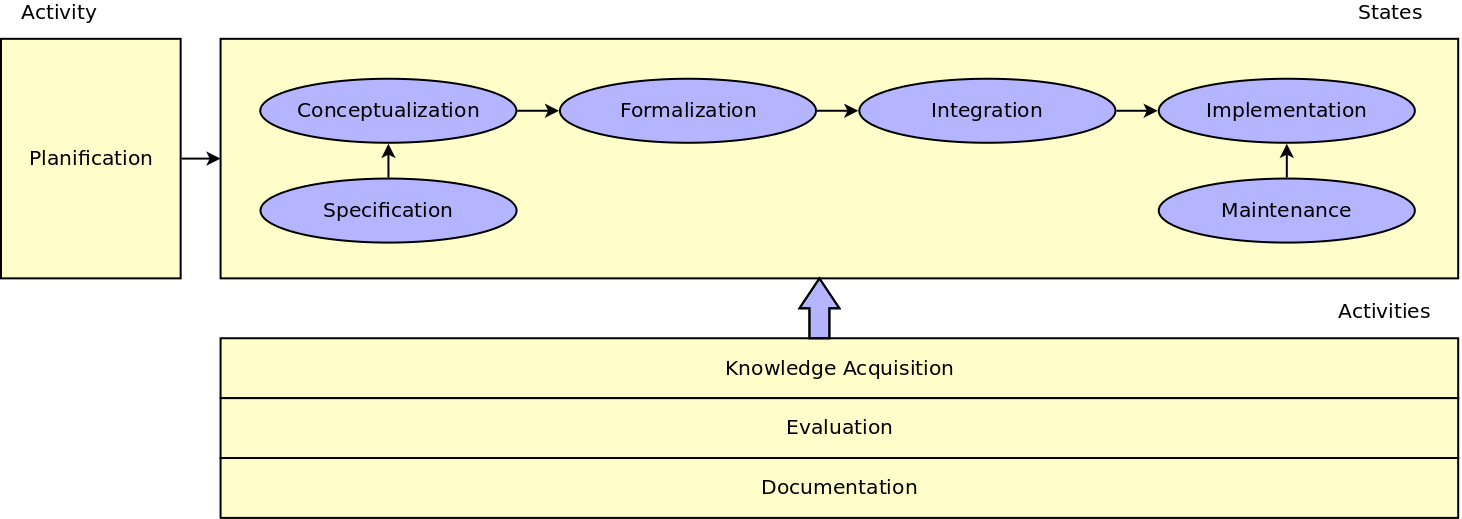
\includegraphics[width=\textwidth]{figures/ontology_lifecycle.pdf}
  \caption{States and activities in the life cycle of an ontology according to \methontology \cite{Methontology}}
  \label{fig:methontology1}
\end{figure}

These activities -- which are depicted in figure \ref{fig:methontology1} -- are arranged into the step of \emph{planification} that must be performed at the very beginning of development, a \emph{set of stages} (consisting of \emph{specification}, \emph{conceptualisation}, \emph{formalisation}, \emph{integration}, \emph{implementation} and \emph{maintenance}) which the ontology moves through during its creation and some activities (\emph{knowledge acquisition}, \emph{documentation} and \emph{evaluation}) that are performed throughout the whole development process in parallel to the stages.

Differently to what is shown in figure \ref{fig:methontology1}, \methontology follows an evolving life cycle model similar to the iterative-incremental approach that is used in the \emph{Spiral Model} in software development\cite{spiral_model}. This life cycle model which allows the ontology to grow according to its needs. Whenever it is necessary, pieces of the ontology can be added, modified and deleted. Thus, one state does not have to be completely finished before the next state is begun. The ontology cycles through each state numerous times until the ontology meets all requirements and the results of each step correspond to each other.

\subsection{The \methontology approach}
\label{sec:methontology}

This section describes \methontology as a well-defined approach to perform all activities mentioned above.

For each of the activities, only ideas behind them are covered, but their application is omitted. They are applied in chapter \ref{ch:smarthomeweather_ontology} where \methontology is used to create the \smarthomeweather ontology.

Each section that describes an activity involving the creation of some documentation artefact (e.g. a table or a document), a template for the respective artefact is presented.

\subsubsection{Specification}
\label{subsec:methontology_specification}

\methontology defines a precise approach for the development of an ontology. It specifies certain activities that need to be performed, how these activities are performed and in which order. Thus, the activity of \emph{planification} is completed by specifying \methontology itself and the ontology developer is exempted therefrom. Hence, the first step of developing an ontology from scratch is \emph{specification}

During \emph{specification}, an \emph{Ontology Requirements Specification Document} is generated. This document is written in natural language using a set of intermediate representations or using competence questions. It should include

\begin{itemize}
  \item the name and the purpose of the ontology, its scope, its intended uses, and possible end-users,
  \item a list of functional requirements (describing the intended functionality of the ontology) and non-functional requirements (describing all intended properties of the ontology not directly related to its functionality), and
  \item a list of terms that specifies the scope of the ontology.
\end{itemize}

A good ontology specification document has the following properties:

Figure~\ref{fig:ontology_specification_template} shows a template of an \emph{Ontology Requirements Specification Document}~\cite{ORSD}.

\begin{figure}
\begin{mdframed}[linewidth=.6pt]
\setlength{\parindent}{0pt}
\MakeUppercase{\textbf{Ontology Requirements Specification Document}}

\textbf{Name}: …

\textbf{Purpose}: …

\textbf{Scope}: …

\textbf{Implementation language}: …

\textbf{Intended end-users}: …

\textbf{Intended uses}: …

\textbf{Ontology requirements}: …

\setlength{\leftskip}{.5cm}

\textbf{Non-functional requirements}: 

\begin{itemize}
  \item …
\end{itemize}

\textbf{Functional requirements}: 

\begin{itemize}
  \item …
\end{itemize}

\setlength{\leftskip}{0cm}

\textbf{Pre-glossary of terms}: …

\end{mdframed}

\caption{Template for the \emph{Ontology Requirements Specification Document} of \methontology~\cite{ORSD}}
\label{fig:ontology_specification_template}
\end{figure}

\subsubsection{Knowledge Acquisition}

Most of knowledge acquisition is done simultanously with the \emph{specification} phase. It is one of the most important activities and needs to be performed thoroughly as most other activities heavily depend on it.

Sources of knowledge are experts, books, handbooks, figures, tables and even other ontologies. Knowledge is collected using techniques such as brainstorming, interviews, formal and informal analysis of texts and knowledge acquisition tools.

\subsubsection{Conceptualisation}
\label{subsec:methontology_conceptualisation}
\begin{figure}
  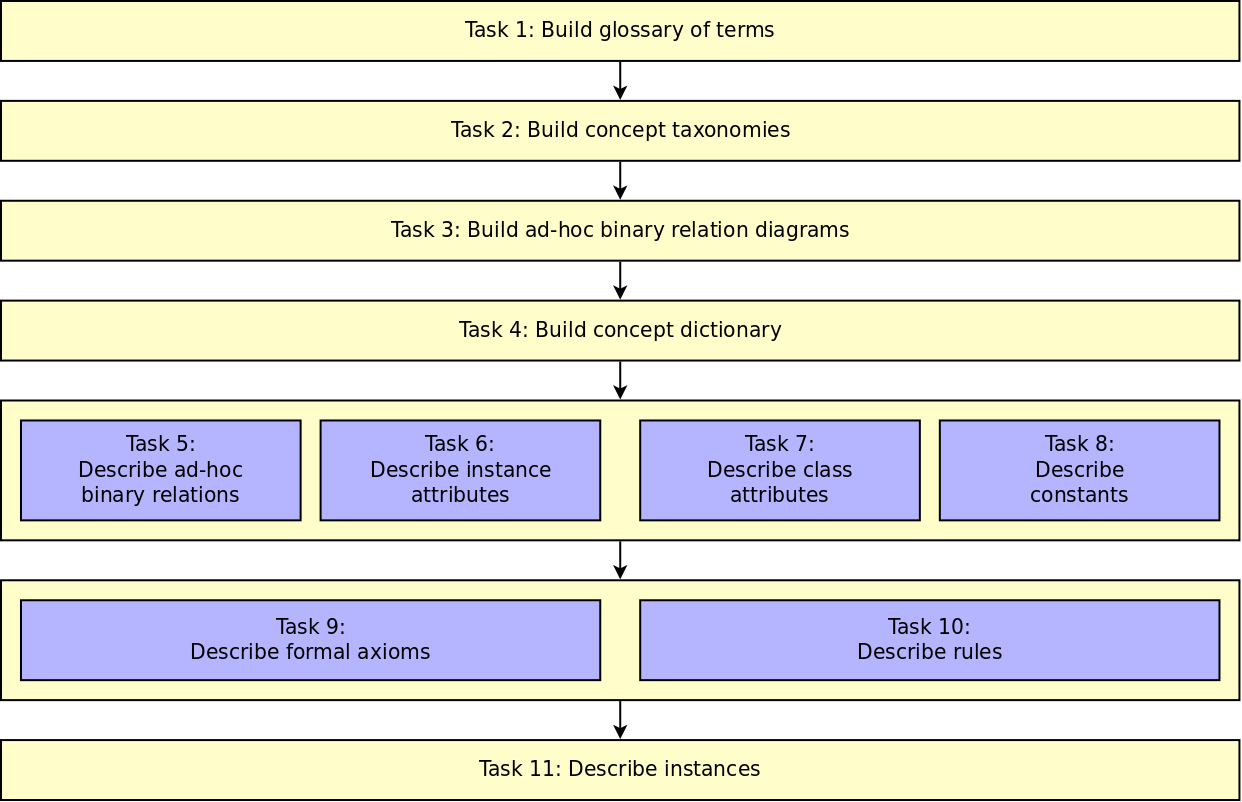
\includegraphics[width=\textwidth]{figures/methontology_tasks.pdf}
  \caption{Tasks of the conceptualisation activity according to \methontology \cite{MethontologyLegal}}
  \label{fig:methontology2}
\end{figure}

The state of \emph{conceptualisation} consists of several tasks as shown in figure \ref{fig:methontology2} \cite{MethontologyLegal}. Again, the figure shows the tasks in a sequential manner. However, as \methontology uses an evolutionary process model, the steps are performed numerous times.

\paragraph{Task 1: Glossary of Terms}

At first, the ontologist builds a \emph{Glossary of Terms}. This glossary includes all the relevant terms of the domain (concepts, instances, attributes, relations etc.). It can be built as a table having the columns \emph{name}, \emph{synonyms}, \emph{acronyms}, \emph{description} (for a natural language description of the term) and \emph{type} (specifying whether the term is a concept, an instance, an attribute, a relation etc.).

\begin{figure}
\centering
\begin{tabular}{|p{.2\textwidth}|p{.2\textwidth}|p{.2\textwidth}|p{.2\textwidth}|}
  \hline
  \textbf{Name} & \textbf{Acronyms} & \textbf{Description} & \textbf{Type} \\
  \hline\hline
  … & … & … & … \\
  \hline
\end{tabular}
\caption{Template for the glossary of terms as proposed by \methontology.}
\label{fig:methontology_example_glossary}
\end{figure}

Figure~\ref{fig:methontology_example_glossary} shows a template for the glossary of terms.

\paragraph{Task 2: Concept Taxonomies}

Once the glossary of terms contains a sizeable number of concepts, these ontologies are arranged in one or more taxonomies that define the concept hierarchy.

\methontology proposes the use of four taxonomic relations:
\begin{enumerate}
  \item \textbf{Subclass-Of}: If a concept $B$ is a \emph{Subclass-Of} a concept $A$, every instance of $B$ is also an instance of $A$.
  \item \textbf{Disjoint-Decomposition}: A \emph{Disjoint-Decomposition} of a concept $C$ is a set of subclasses of $C$ such that an instance of one of these subclasses can never be a subclass of another of these subclasses, while an instance of $C$ is not necessarily an instance of one of its subclasses.
  \item \textbf{Exhaustive-Decomposition}: A \emph{Exhaustive-Decomposition} of a concept $C$ is a set of subclasses of $C$ such that every instance of $C$ is an instance of at least one of its subclasses.
  \item \textbf{Partition}: A \emph{Partition} of $C$ is a set of subclasses of $C$ such that every instance of $C$ is an instance of exactly one of its subclasses.
\end{enumerate}

\begin{figure}
\centering
\includegraphics[width=.9\textwidth]{figures/diagrams/methontology_example_concept_taxonomies.pdf}
\caption{Example of a concept-classification tree as proposed by \methontology.}
\label{fig:methontology_example_concept_taxonomies}
\end{figure}

The concept taxonomies are visualised in \emph{concept-classification trees} which are diagrams that depict the concepts and their taxonomic relations. See figure~\ref{fig:methontology_example_concept_taxonomies} for an example of a concept-classification tree. In case the ontology contains a large number of concepts, the tree may be split into several diagrams in order to keep the trees clear.

\paragraph{Task 3: Ad-hoc binary relation diagrams}

In the next step, \emph{ad-hoc binary relation diagrams} are created. This diagrams show all ad-hoc relationships between concepts of the same (or different) concept taxonomies. See figure~\ref{fig:methontology_example_binary_relations} for an example of a binary relation diagram.

\begin{figure}
\centering
\includegraphics[width=.8\textwidth]{figures/diagrams/methontology_example_binary_relations.pdf}
\caption{Example of a binary relations diagram as proposed by \methontology.}
\label{fig:methontology_example_binary_relations}
\end{figure}

\paragraph{Task 4: Concept dictionary}

The \emph{concept dictionary} contains all domain concepts together with their relations, their instances and their class attributes (i.e. attributes that describe properties of classes) and instance attributes (i.e. attributes that describe properties of instances). All information from the previous steps contribute to this dictionary. The concept dictionary is again being built as a table having appropriate columns for all required information. Like the concept-classification trees, this table may be split into a set of smaller tables if the ontology contains a large number of concepts.

Figure~\ref{fig:methontology_example_concept_dictionary} shows a template for the concept dictionary.

\begin{figure}
\centering
\begin{tabular}{|p{.2\textwidth}|p{.5\textwidth}|p{.2\textwidth}|}
  \hline
  \textbf{Name} & \textbf{Instances} & \textbf{Relations} \\
  \hline\hline
  … & … & … \\
  \hline
\end{tabular}
\caption{Template for the concept dictionary as proposed by \methontology.}
\label{fig:methontology_example_concept_dictionary}
\end{figure}

\paragraph{Task 5: Ad-hoc binary relation details}

In this step, for all ad-hoc binary relations details are specified in a tabular manner. The resulting table has a row for each relation and columns named \emph{relation name}, \emph{source concept}, \emph{source cardinality (max)}, \emph{target concept}, \emph{inverse relation}. Figure~\ref{fig:methontology_example_binary_relations_table} shows a template for the binary relations table.

\begin{figure}
\centering
\begin{tabular}{|p{.167\textwidth}|p{.167\textwidth}|p{.167\textwidth}|p{.167\textwidth}|p{.167\textwidth}|}
  \hline
  \textbf{Name} & \textbf{Source\newline concept} & \textbf{Target\newline concept} & \textbf{Maximum\newline source\newline cardinality} & \textbf{Inverse\newline relation} \\
  \hline\hline
  … & … & … & … & … \\
  \hline
\end{tabular}
\caption{Template for the binary relations table as proposed by \methontology.}
\label{fig:methontology_example_binary_relations_table}
\end{figure}

\paragraph{Task 6: Instance attributes}

This step leads to an \emph{instance attributes table}. That is a table of all \emph{instance attributes} that are listed in the concept dictionary. Each row contains the description of one instance attribute. An instance attribute is an attribute that describes a property of an instance of a concept. Its value may be different for each instance of the concept.

The columns of the table are \emph{attribute name}, \emph{concept name}, \emph{value type} (\emph{Integer}, \emph{Float}, \emph{String}, etc.), \emph{value range}, \emph{minimum cardinality} and \emph{maximum cardinality}. Additionally, the following information may be specified: instance attributes, class attributes and constants used to infer values of the attribute; attributes that can be inferred using values of this attribute; formulae or rules that allow inferring values of the attribute; and references used to define the attribute.

See figure~\ref{fig:methontology_example_instance_attributes} for a template for the instance attributes table.

\begin{figure}
\centering
\begin{tabular}{|p{0.15\textwidth}|p{0.15\textwidth}|p{0.15\textwidth}|p{0.15\textwidth}|p{0.15\textwidth}|p{0.15\textwidth}|}
  \hline
  \textbf{Attribute name} & \textbf{Concept name} & \textbf{Value type} & \textbf{Value range} & \textbf{Unit} & \textbf{Cardinality} (min, max)\\
  \hline\hline
  … & … & … & … & … & … \\
  \hline
\end{tabular}
\caption{Template for the instance attributes table as proposed by \methontology.}
\label{fig:methontology_example_instance_attributes}
\end{figure}

\paragraph{Task 7: Class attributes}

All class attributes that are listed in the concept dictionary are described in detail in the \emph{class attributes table}. Each row describes one class attribute. The columns are \emph{name}, \emph{concept name} (i.e. the name of the concept where the attribute is defined), \emph{value type}, \emph{value(s)}, \emph{minimum cardinality} and \emph{maximum cardinality}. Additionally, all information about related instance attributes, class attributes, constants, rules, and formulae may be specified that are specified in the instance attribute as well.

\begin{figure}
\centering
\begin{tabular}{|p{0.22\textwidth}|p{0.22\textwidth}|p{0.22\textwidth}|p{0.22\textwidth}|}
  \hline
  \textbf{Super-concept} & \textbf{Sub-concept} & \textbf{attribute name} & \textbf{attribute value(s)} \\
  \hline\hline
  … & … & … & … \\
  \hline
\end{tabular}
\caption{Template for the class attributes table as proposed by \methontology.}
\label{fig:methontology_example_class_attributes}
\end{figure}

Figure~\ref{fig:methontology_example_class_attributes} shows a template for the class attributes table.

\paragraph{Task 8: Constants}

In this step, the \emph{constants table} is created that specifies details about all the constants listed in the glossary of terms. Each constant is specified by its name, its value type, its value, the measurement unit for numerical constants, and the attributes that can be inferred using the constant.

\begin{figure}
\centering
\begin{tabular}{|p{0.2\textwidth}|p{0.2\textwidth}|p{0.2\textwidth}|p{0.2\textwidth}|}
  \hline
  \textbf{Constant name} & \textbf{Value type} & \textbf{Value} & \textbf{Measurement unit} \\
  \hline\hline
  … & … & … & … \\
  \hline
\end{tabular}
\caption{Template for the constants table as proposed by \methontology.}
\label{fig:methontology_example_constants}
\end{figure}

Figure~\ref{fig:methontology_example_constants} shows a template for the constants table.

\paragraph{Task 9: Formal axioms}

In this task, the ontology designer must determine whether the ontology contains formal axioms. In case it contains any, these axioms must be defined precisely in a \emph{formal axioms table}. For each axiom, this table specifies the name, a description in natural language, the logical expression that formally describes the axiom in first-order logic (or the logic the ontology language intended to use is based upon), and all concepts, attributes, relations, and variables that are referred to in the logical expression. Figure~\ref{fig:methontology_example_axioms} presents a template for the formal axioms table.

\begin{figure}
\centering
\begin{tabularx}{\textwidth}{|X|X|X|X|X|X|X|}
  \hline
  \textbf{Axiom name} & \textbf{Description} & \textbf{Expression} & \textbf{Referred\newline concepts} & \textbf{Referred\newline attributes} & \textbf{Referred\newline relations} & \textbf{Variables} \\
  \hline\hline
  … & … & … & … & … & … & … \\
  \hline
\end{tabularx}
\caption{Template for the formal axioms table as proposed by \methontology.}
\label{fig:methontology_example_axioms}
\end{figure}

\paragraph{Task 10: Rules}

Similary to the task of identifying and describing formal axioms within the ontology, in this step the ontology designer must determine whether the ontology contains any rules. If it contains any, a \emph{rules table} must be built to precisely describe all rules and their properties: Their name, their description, an expression in first-order logic, and all concepts, attributes, relations, and variables involved. In contrast to formal axioms, the expression of rules always has the form \emph{if <conditions> then <consequent>}; hereby \emph{<conditions>} is a conjunction of atoms while \emph{<consequent>} is a single atom.

For the rules table, the template for the formal axioms table (see figure~\ref{fig:methontology_example_axioms}) can be reused.

\paragraph{Task 11: Instances}

Within an ontology, a set of instances may be predefined. This task involves listing these individuals, again in tabular manner. The columns of this \emph{instances table} are the name of the instance, the name of the concept and all of the instance's attributes together with their respective values. Figure~\ref{fig:methontology_example_instances} depicts a template for the instances table.

\begin{figure}
\centering
\begin{tabular}{|p{0.2\textwidth}|p{0.2\textwidth}|p{0.2\textwidth}|p{0.2\textwidth}|}
  \hline
  \textbf{Instance name} & \textbf{Concept name} & \textbf{Attribute} & \textbf{Value(s)} \\
  \hline\hline
  … & … & … & … \\
  \hline
\end{tabular}
\caption{Template for the instants table as proposed by \methontology.}
\label{fig:methontology_example_instances}
\end{figure}

\subsubsection{Formalisation}

\emph{Formalisation} is the transition from the informal description of the tables and diagrams in the previous step of \emph{conceptualisation} into the chosen ontology language, e.g. \eacs{OWL}. As this is tightly coupled with the \emph{implementation} of the ontology (see section~\ref{subsec:methontology_implementation}), this is a task which is not performed separately.

\subsubsection{Integration}

As ontologies are built for reuse and the wheel shall not be reinvented during the creation of a new ontology, the ontology designer searches for existing ontologies. The goal is to import ontologies that already define terms that are part of the conceptualisation currently being developed.

\subsubsection{Implementation}
\label{subsec:methontology_implementation}

The task of implementing the ontology in an ontology language requires an environment that supports the ontologies selected in the integration step. Features that should be provided by such an environment are~\cite{Methontology}:

\begin{itemize}
  \item a lexical and syntactic analyser to guarantee the absence of lexical and syntactic errors,
  \item an editor for adding, modifying and removing definitions,
  \item a browser for inspecting the library of ontologies and their definitions,
  \item a searcher for looking for the most appropriate definitions,
  \item evaluators for detecting incompleteness, inconsistencies and redundant knowledge and
  \item an automatic maintainer for managing the inclusion, removal or modification of existing definitions.
\end{itemize}

Together with the implementation, the information about the ontology gathered during the process described in section~\ref{subsec:methontology_conceptualisation} is now formalised into the formal model of the ontology language being used.

In the case of the \smarthomeweather ontology an \eacs{OWL} ontology~\cite{OWL} is created using \protege~\cite{protege} together with the \emph{Pellet} reasoner~\cite{pellet}.

\subsubsection{Evaluation}

During \emph{Evaluation}, verification takes place whether all artefacts that have yet been created or updated in the previous steps satisfy the requirements that have been initially). \emph{Evaluation} is not an activity which is performed at the very end of the development process; instead, \emph{Evaluation} takes place whenever an artefact (a diagram, a table, or the implementation of the ontology) is created or updated in order to ensure that mistakes are found as soon as possible.

The completed ontology must fulfil all functional and non-functional requirements listed the \emph{Ontology Requirements Specification Document} presented in section~\ref{subsec:methontology_specification}. In case of a mismatch, the ontology traverses the activities of the life cycle (\emph{Conceptualisation}, \emph{Formalisation}, \emph{Integration}, \emph{Implementation}, and \emph{Evaluation}) once more.

There may be requirements that an ontology is unable to fulfil due to certain limitations, e.g. the \emph{open world assumption}~\cite{open_world_assumption1}. For instance, \eacs{OWL}, which honors the \emph{open world assumption}, cannot tell the absence of an instance of some concept. This leads to cases where an ontology fails to answer a competency question such as ``Does this group only consist of women?''; just because the ontology does not contain an individual which is a man, it does not mean that there is no man; the ontology can only tell that there is no man it knows about.

Evaluation (and specification) must hereby take limitations into account which affect ontologies or the ontology language being used.

\subsubsection{Documentation}

During the steps described above, a set of documents is compiled. If generated properly and accurately, these documents describe every detail of the ontology. Using this approach, \methontology forces the ontology designer to document throughout the development process. Any problems that come with incomplete or wrong documentation are avoided~\cite{SoftwareDocumentationProblems}.

Hence, in \methontology, \emph{documentation} is an activity that is not performed explicitly. Once the development process has finished, both the ontology and its documentation are ready to use. 

\subsubsection{Maintenance}

At any time in the future, changes to the ontology may become necessary. A modification of the ontology's requirements may be one reason therefor; inaccurateness that occurred during the ontology development process may be another reason.

Whenever a change is necessary, the ontology again cycles the states of \emph{specification}, \emph{conceptualisation}, \emph{formalisation}, \emph{integration} and \emph{implementation} repeatedly until all requirements are met and all artefacts generated in these states correspond to each other. \emph{Knowledge acquisition} and \emph{evaluation} are also again performed throughout all of these states.

% TODO new section: conclusion